% Standalone Fig. 2: scalar encoding (top) and record layout (bottom).
% The manuscript still inputs record_layout_update4.tex; this file is separate.
% Facts follow evidence/record-example.json: kernel-order scalars 0-2 are
% 3C12/3956/4178, with codes 000/111/111, escape selectors 0001/1111 (packed
% into byte F1), and raw patch (escape index 1, high byte 41). Low 16 KiB,
% codes 6 KiB, variable region 64 B = 48 + 1 + 3 + 4 + 8. Widths are not to
% scale. Coordinates are final-size points (252 pt = \columnwidth); y grows
% downward. The 114.5 pt height keeps the current four-page layout together
% with images/figure2-record-split-caption.txt.
% Export: python3 paper/render_figures.py --figures 2 \
%   --source figures/record_layout_split.tex --output-stem figure2-record-split
\definecolor{rsInk}{HTML}{202C3A}%
\definecolor{rsMuted}{HTML}{586779}%
\definecolor{rsRule}{HTML}{D5DCE4}%
\definecolor{rsFrame}{HTML}{AAB8C7}%
\definecolor{rsPad}{HTML}{E9EDF2}%
\definecolor{rsBlue}{HTML}{246AC0}%
\definecolor{rsBlueTint}{HTML}{EDF4FC}%
\definecolor{rsTeal}{HTML}{00798C}%
\definecolor{rsTealTint}{HTML}{E8F7F9}%
\definecolor{rsOrange}{HTML}{C76821}%
\definecolor{rsOrangeTint}{HTML}{FFF4E8}%
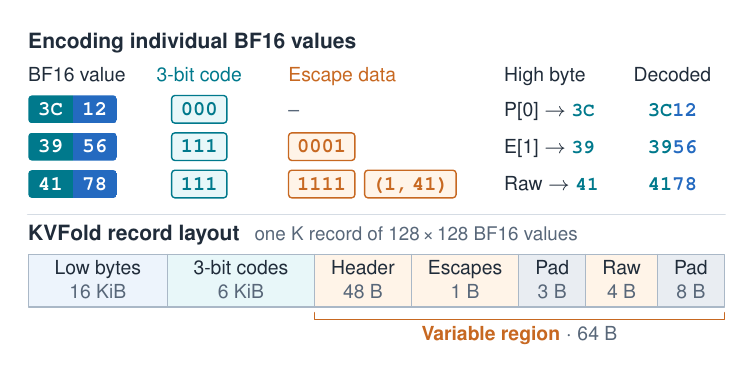
\begin{tikzpicture}[x=1pt,y=-1pt,line cap=round,line join=round,
    every node/.style={inner sep=0pt,text=rsInk,
      font=\fontfamily{phv}\fontsize{7}{8.4}\selectfont},
    mono/.style={font=\fontfamily{pcr}\fontseries{b}\fontsize{7.4}{8.4}\selectfont},
    title/.style={anchor=base west,
      font=\fontfamily{phv}\fontseries{b}\fontsize{7.6}{9}\selectfont},
    note/.style={text=rsMuted,font=\fontfamily{phv}\fontsize{6.8}{8}\selectfont},
    chip/.style={mono,draw,rounded corners=1.2pt,line width=.5pt,
      minimum height=10pt,inner xsep=2.6pt,text height=4.4pt,text depth=0pt},
    code/.style={chip,fill=rsTealTint,draw=rsTeal,text=rsTeal},
    esc/.style={chip,fill=rsOrangeTint,draw=rsOrange,text=rsOrange}]
  \path[use as bounding box] (0,0) rectangle (252,114.5);

  % #1 row centre, #2 high byte, #3 low byte: one solid two-byte BF16 value.
  \def\rsValue#1#2#3{%
    \begin{scope}
      \clip[rounded corners=1.2pt] (.25,#1-5) rectangle (32.25,#1+5);
      \fill[rsTeal] (.25,#1-5) rectangle (16.25,#1+5);
      \fill[rsBlue] (16.25,#1-5) rectangle (32.25,#1+5);
    \end{scope}
    \node[mono,text=white,text height=4.4pt,text depth=0pt] at (8.25,#1) {#2};
    \node[mono,text=white,text height=4.4pt,text depth=0pt] at (24.25,#1) {#3};}
  % #1 row centre, #2 table entry or Raw, #3 high byte, #4 low byte.
  \def\rsDecode#1#2#3#4{%
    \node[anchor=base west] at (172,#1+2.5)
      {#2 $\rightarrow$ {\fontfamily{pcr}\fontseries{b}\selectfont\color{rsTeal}#3}};
    \node[anchor=base,mono] at (233,#1+2.5)
      {\color{rsTeal}#3\color{rsBlue}#4};}
  % #1 left, #2 right, #3 fill, #4 field name, #5 size: one record field.
  \def\rsField#1#2#3#4#5{%
    \fill[#3] (#1,82) rectangle (#2,101);
    \node[anchor=base] at ({(#1+#2)/2},89.3) {#4};
    \node[anchor=base,text=rsMuted] at ({(#1+#2)/2},97.7) {#5};}

  % --- Top: three example values; each row is one complete encode/decode path.
  \node[title] at (0,7.6) {Encoding individual BF16 values};
  \node[anchor=base west] at (0,19.5) {BF16 value};
  \node[anchor=base,text=rsTeal] at (62,19.5) {3-bit code};
  \node[anchor=base west,text=rsOrange] at (94,19.5) {Escape data};
  \node[anchor=base west] at (172,19.5) {High byte};
  \node[anchor=base] at (233,19.5) {Decoded};

  \rsValue{29.5}{3C}{12}
  \node[code,minimum width=20pt] at (62,29.5) {000};
  \node[anchor=base west,text=rsMuted] at (94,32) {--};
  \rsDecode{29.5}{P[0]}{3C}{12}

  \rsValue{43}{39}{56}
  \node[code,minimum width=20pt] at (62,43) {111};
  \node[esc,minimum width=24pt,anchor=west] at (94,43) {0001};
  \rsDecode{43}{E[1]}{39}{56}

  \rsValue{56.5}{41}{78}
  \node[code,minimum width=20pt] at (62,56.5) {111};
  \node[esc,minimum width=24pt,anchor=west] (raw) at (94,56.5) {1111};
  \node[esc,anchor=west] at ([xshift=3pt]raw.east) {(1,\,41)};
  \rsDecode{56.5}{Raw}{41}{78}

  \draw[rsRule,line width=.5pt] (0,67.5) -- (252,67.5);

  % --- Bottom: the record as one bar. Every field shows its name and size;
  % the bracket groups the five fields of the variable region.
  \node[title] (rtitle) at (0,77) {KVFold record layout};
  \node[note,anchor=base west] at ([xshift=5pt]rtitle.base east)
    {one K record of 128\,\texttimes\,128 BF16 values};

  \rsField{.25}{50.45}{rsBlueTint}{Low bytes}{16 KiB}
  \rsField{50.45}{103.65}{rsTealTint}{3-bit codes}{6 KiB}
  \rsField{103.65}{138.65}{rsOrangeTint}{Header}{48 B}
  \rsField{138.65}{177.45}{rsOrangeTint}{Escapes}{1 B}
  \rsField{177.45}{201.65}{rsPad}{Pad}{3 B}
  \rsField{201.65}{227.55}{rsOrangeTint}{Raw}{4 B}
  \rsField{227.55}{251.75}{rsPad}{Pad}{8 B}
  \draw[rsFrame,line width=.5pt] (.25,82) rectangle (251.75,101);
  \foreach \x in {50.45,103.65,138.65,177.45,201.65,227.55}
    \draw[rsFrame,line width=.5pt] (\x,82) -- (\x,101);

  \draw[rsOrange,line width=.6pt] (103.65,103) -- (103.65,105.5)
    -- (251.75,105.5) -- (251.75,103);
  \node[anchor=base] at (177.7,113.2)
    {{\fontseries{b}\selectfont\color{rsOrange}Variable region}
     {\color{rsMuted}$\cdot$ 64 B}};
\end{tikzpicture}%
